%!TEX root = ../Thesis.tex

\section{Numerical Implementation of the BEM}
\label{sec:numerical_implementation_of_the_bem}%

Let us consider the case where $f=0$. The quintessence of the BEM is to discretize the boundary $\Gamma$ into a finite number of segments which are called \emph{boundary elements}. Two approximations are made over each of these elements. One concerns the geometry of the boundary, while the other has to do with the variation of the unknown boundary quantity over the element. Here we choose the simplest approach, which means that our boundary element is a \emph{constant element}: the boundary segment is approximated by a straight line which connects the two \emph{end points}, and then we place a \emph{nodal point} at the midpoint of the line. In other words, the boundary quantity is assumed to be constant along the element and equal to its value at the nodal point (see Figure~\ref{fig:costant}).

\begin{figure}[H]
  \centering
    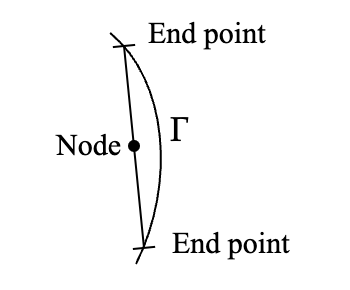
\includegraphics[width=0.3\textwidth]{costantBEM}
    \caption{Approximation of the boundary segment by a constant element.} 
    \label{fig:costant}
\end{figure}

\subsection{BEM with constant elements for the Laplace Equation}
\label{sub:bem_with_constant_elements}%

The boundary $\Gamma$ is discretized into $N$ constant elements numbered in counter-clockwise sense. Therefore the discretized version of Eq.~\eqref{eq:bie} for a given point $\yv_i$ on $\Gamma$ is 
\begin{equation}
\label{eq:bem1}
\frac{1}{2}\ u^i =-\sum_{j=1}^N \int_{\Gamma_j} \frac{\partial u}{\partial n}(\mathbf{x})\ G(\mathbf{x},\mathbf{y}_i)\ \mathrm{d}S(\mathbf{x}) +\sum_{j=1}^N \int_{\Gamma_j} \frac{\partial G}{\partial n}(\mathbf{x},\mathbf{y}_i)\ u(\mathbf{x}) \ \mathrm{d}S(\mathbf{x}).
\end{equation}

Since the values of $u$ and $\partial u / \partial n$ are constant on each element, they can be moved outside the integral. Then Eq.~\eqref{eq:bem1} may be written as
\begin{equation}
\label{eq:bem2}
-\frac{1}{2}\ u^i +\sum_{j=1}^N \underbracket[0.5pt]{\left( \int_{\Gamma_j} \frac{\partial G}{\partial n}\ \mathrm{d}S \right)}_{\hat{H}_{ij}} u^j=\sum_{j=1}^N \underbracket[0.5pt]{\left( \int_{\Gamma_j} G\ \mathrm{d}S \right)}_{G_{ij}}u_n^j
\end{equation}

Simply setting 
\begin{equation*}
H_{ij}=\hat{H}_{ij}-\frac{1}{2}\,\delta_{ij},
\end{equation*}
where $\delta_{ij}$ is the \emph{Kronecker delta}, Eq.~\eqref{eq:bem2} becomes
\begin{equation}
\label{eq:bem3}
\sum_{j=1}^N H_{ij}\,u^j=\sum_{j=1}^N G_{ij}\,u^j_n.
\end{equation}

We apply Equation~\eqref{eq:bem3} to all nodes $\yv_i$ for $i=1,\dots,N$ and we finally obtain a system of $N$ linear algebraic equations, which are arranged in matrix form
\begin{equation}
\label{eq:bem4}
Hu=Gu_n,\qquad H,\,G\in\RR^{N\times N},\qquad u,\,u_n\in\RR^{N\times 1}.
\end{equation}

Since we have mixed boundary conditions~\eqref{eq:laplace-problem}, we need to decouple the system by separating the unknown from the known quantities. This leads to a final $N \times N$ system in the form 
\begin{equation}
\label{eq:finalAx=b}
Ax=b, 
\end{equation}
where $x=(u\text{ on }\Gamma_2,\ u_n\text{ on }\Gamma_1)'$ groups the unknowns.

Once the boundary quantities $u$ and $u_n$ are known, the solution $u$ can be computed at any point $\yv$ inside the domain $\Omega$ using Eq.~\eqref{eq:solid-angle}
\begin{equation}
u(\yv)=\sum_{j=1}^N \hat{H}_{ij}\,u^j-\sum_{j=1}^N G_{ij}\,u^j_n
\end{equation}

and by direct differentiation we can obtain its gradient.

\subsection{Line integrals and BEM for the Poisson Equation}
\label{sub:line_integrals_and}%

We mention that the line integrals $G_{ij}$ and $\hat{H}_{ij}$ are evaluated numerically using a standard Gaussian quadrature. Moreover, the Poisson version of system~\eqref{eq:bem4} is
\begin{equation}
\label{eq:bem5}
Hu+F=Gu_n,
\end{equation}

where the term $F$ contains the evaluation of the domain integrals~\eqref{eq:PassoAsso} by employing two-dimensional Gaussian integration. For further explanations, see~\cite{sbemKatsi}.

\bigskip

\bigskip

On the basis of the analysis presented so far, we are going to present and solve three problems ruled by the Laplace equation. Then we will compare our MATLAB and Abaqus results, as well as with the ones obtained using FORTRAN in~\cite{sbemKatsi}. 

\newpage






